\chapter{Экспериментальная часть}
\label{cha:research}

В данной части будет проведена апробация и тестирование разработанной программы.

\section{Примеры работы}

% примеры со скриншотами интерфейса
Программа имеет консольный интерфейс. Далее будут приведены скриншоты.

На рис. \ref{screenshot-usage} показаны возможные сценарии запуска программы.

\begin{figure}
    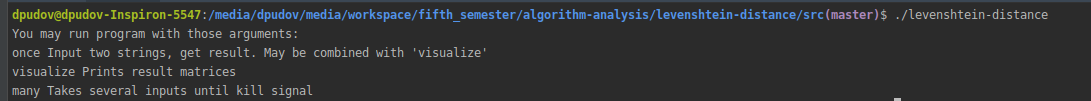
\includegraphics[width=0.9\textwidth]{screenshots/screenshot-usage}
    \caption{Использование программы.}
    \label{screenshot-usage}
\end{figure}

На рис. \ref{screenshot-once} показан пример использования программы с однократным вводом входных данных.

\begin{figure}
    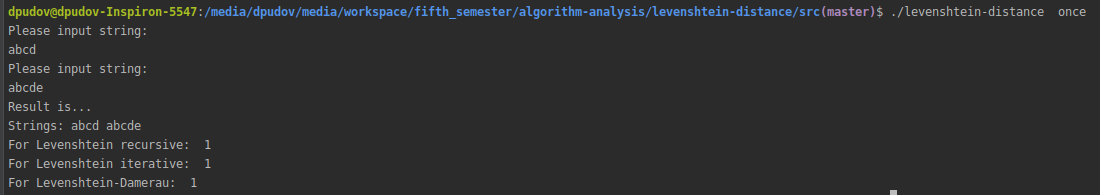
\includegraphics[width=0.9\textwidth]{screenshots/screenshot-once}
    \caption{Однократное использование.}
    \label{screenshot-once}
\end{figure}

На рис. \ref{screenshot-visualize} показан пример использования программы с выводом матриц.

\begin{figure}
    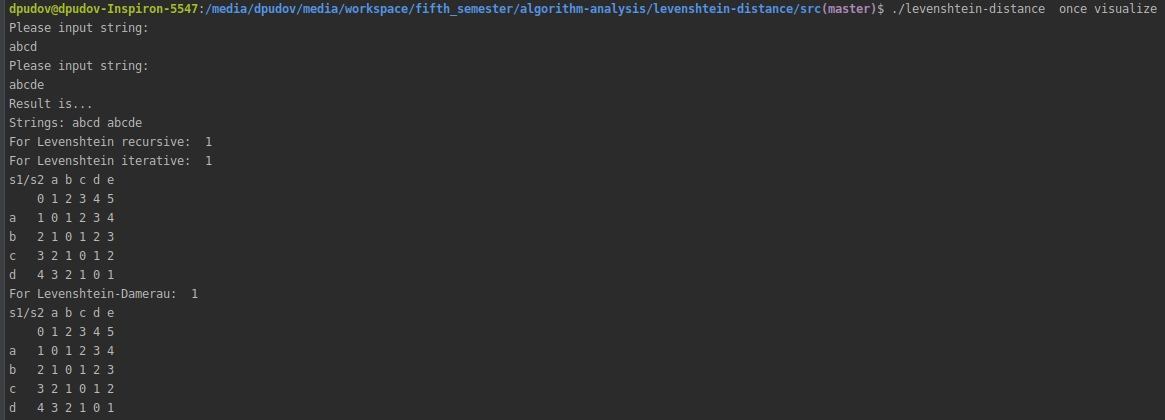
\includegraphics[width=0.9\textwidth]{screenshots/screenshot-visualize}
    \caption{Использование с выводом матриц.}
    \label{screenshot-visualize}
\end{figure}

На рис. \ref{screenshot-many} показан пример использования программы со множеством входных данных.

\begin{figure}
    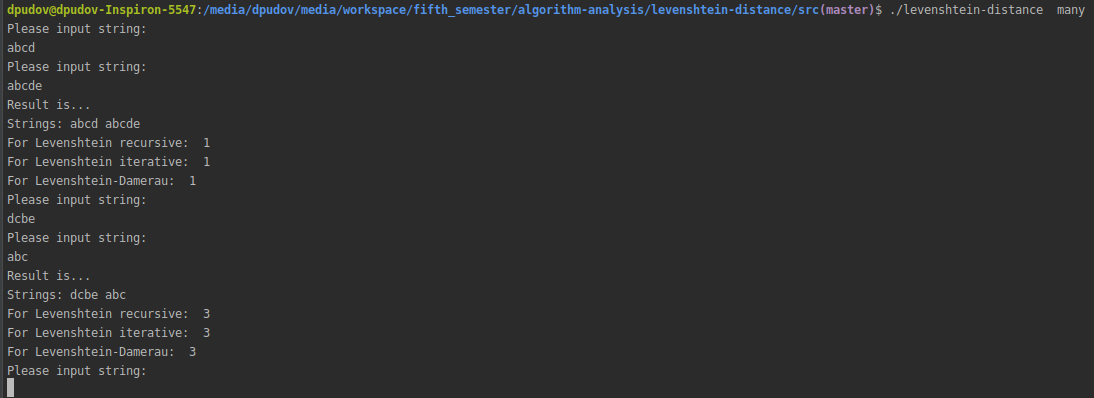
\includegraphics[width=0.9\textwidth]{screenshots/screenshot-many}
    \caption{Многократное использование.}
    \label{screenshot-many}
\end{figure}

\FloatBarrier

\section{Результаты тестирования}

В данном разделе будут расположены результаты тестирования ранее описанных
реализаций.

В табл. \ref{table-testing-results-recursive} отражены результаты тестирования рекурсивной
реализации алгоритма поиска расстояния Левенштейна.

\begin{table}
    \caption{Результаты тестирования рекурсивной реализации.}
    \label{table-testing-results-recursive}
    \begin{center}
        \begin{tabular}{|c|c|c|c|}
            \hline
            S1 & S2 & Ожидаемый результат & Фактический результат \\
            \hline
            Пустая строка & Пустая строка & 0 & 0\\
            \hline
            "abc" & "abc" & 0 & 0\\
            \hline
            "abc" & "def" & 3 & 3\\
            \hline
            "abcdef" & "abc" & 3 & 3\\
            \hline
            "abc" & "abcdef" & 3 & 3\\
            \hline
            "xyzabc" & "abcdef" & 6 & 6\\
            \hline
            "abkdef" & "abcdefg" & 2 & 2\\
            \hline
            "abc" & "acb" & 2 & 2\\
            \hline
        \end{tabular}
    \end{center}
\end{table}

В табл. \ref{table-testing-results-iterative} отражены результаты тестирования матричной
реализации алгоритма поиска расстояния Левенштейна.

\begin{table}
    \caption{Результаты тестирования матричной реализации.}
    \label{table-testing-results-iterative}
    \begin{center}
        \begin{tabular}{|c|c|c|c|}
            \hline
            S1 & S2 & Ожидаемый результат & Фактический результат \\
            \hline
            Пустая строка & Пустая строка & 0 & 0\\
            \hline
            "abc" & "abc" & 0 & 0\\
            \hline
            "abc" & "def" & 3 & 3\\
            \hline
            "abcdef" & "abc" & 3 & 3\\
            \hline
            "abc" & "abcdef" & 3 & 3\\
            \hline
            "xyzabc" & "abcdef" & 6 & 6\\
            \hline
            "abkdef" & "abcdefg" & 2 & 2\\
            \hline
            "abc" & "acb" & 2 & 2\\
            \hline
        \end{tabular}
    \end{center}
\end{table}

В табл. \ref{table-testing-results-damerau} отражены результаты тестирования матричной
реализации алгоритма поиска расстояния Дамерау-Левенштейна.

\begin{table}
    \caption{Результаты тестирования матричной реализации Дамерау-Левенштейна.}
    \label{table-testing-results-damerau}
    \begin{center}
        \begin{tabular}{|c|c|c|c|}
            \hline
            S1 & S2 & Ожидаемый результат & Фактический результат \\
            \hline
            Пустая строка & Пустая строка & 0 & 0\\
            \hline
            "abc" & "abc" & 0 & 0\\
            \hline
            "abc" & "def" & 3 & 3\\
            \hline
            "abcdef" & "abc" & 3 & 3\\
            \hline
            "abc" & "abcdef" & 3 & 3\\
            \hline
            "xyzabc" & "abcdef" & 6 & 6\\
            \hline
            "abkdef" & "abcdefg" & 2 & 2\\
            \hline
            "abc" & "acb" & 1 & 1\\
            \hline
        \end{tabular}
    \end{center}
\end{table}

\FloatBarrier

\section{Постановка эксперимента по замеру времени и памяти}

Для матричных алгоритмов эксперимент ставился со следующими условиями:
\begin{itemize}
    \item число повторов эксперимента - 100
    \item диапазоны сравниваемых строк: от 100 до 1000 с шагом 100
    \item все строки получены случайным образом.
\end{itemize}

Для рекурсивного алгоритма время на одну итерацию достигает 1.75 мс, при длине строки в 12 символов. Аналогичный эксперимент для матричных реализаций занимает
4 мкс. Поэтому рекурсивная реализация была исключена из дальнейшего исследования.

\section{Сравнительный анализ на материале экспериментальных\\ данных}

% Эксперименты + выводы
В данном разделе будут приведены результаты экспериментов.

Далее приведены сравнительные характеристики матричных реализаций.

\begin{tikzpicture}
\begin{axis}[
    title={Затрачиваемое время на одну итерацию эксперимента\\},
    xlabel={Количество элементов},
    ylabel={Время ns/op}
    ]
    \addplot table [x={count}, y={ns/op}] {
        count               ns/op
            100           301309
            200          1288880
            300          3582494
            400         6036234
            500         12011538
            600         14316484
            700         21022893
            800         32453343
            900         53211084
           1000         65423273
    };
    \addplot table [x={count}, y={ns/op}] {
        count               ns/op
            100           361747
            200          1659175
            300          4241782
            400         7307483
            500         14065218
            600         17071562
            700         24813714
            800         35378085
            900         61728942
           1000         78166044
    };
\end{axis}
\end{tikzpicture}

\begin{tikzpicture}
\begin{axis}[
    title ={Затрачиваемая память на одну итерацию эксперимента\\},
    xlabel={Количество элементов},
    ylabel={Использование памяти B/op}
    ]
    \addplot table [x={count}, y={B/op}] {
        count               B/op
            100           93184
            200          365056
            300          817280
            400         1395585
            500         2064384
            600         2939649
            700         4325377
            800         5249412
            900         7402754
           1000         8224771
    };
    \addplot table [x={count}, y={B/op},
    xlabel={Количество элементов},
    ylabel={Использование памяти B/op}] {
        count               B/op
            100           93184
            200          365056
            300          817280
            400         1395584
            500         2064384
            600         2939653
            700         4325376
            800         5249408
            900         7402755
           1000         8224768
    };
\end{axis}
\end{tikzpicture}

\section{Выводы}

Использование памяти матричными реализациями алгоритмов нахождения расстояний Левенштейна и Дамерау-Левенштейна примерно одинаково, поскольку размерность матрицы одна и та же.

По времени матричный алгоритм поиска расстояния Дамерау-Левенштейна медленнее матричного алгоритма Левенштейна за счёт дополнительного условия на штраф за транспозицию.
